\documentclass[journal,12pt,twocolumn]{IEEEtran}
\makeatletter
\@addtoreset{figure}{problem}
\makeatother
\usepackage{setspace}
\usepackage{gensymb}
\usepackage{xcolor}
\usepackage{caption}
%\usepackage{multirow}
%\usepackage{multicolumn}
%\usepackage{subcaption}
%\doublespacing
\singlespacing
\usepackage{amsmath}
\usepackage{multicol}
\usepackage{enumerate}
\usepackage{amssymb}
%\usepackage{iithtlc}
\usepackage{graphicx}
\usepackage{newfloat}
%\usepackage{syntax}
\usepackage{listings}
\usepackage{color}
\usepackage{tikz}
\usepackage[american]{circuitikz}
\usetikzlibrary{shapes,arrows}



%\usepackage{graphicx}
%\usepackage{amssymb}
%\usepackage{relsize}
%\usepackage[cmex10]{amsmath}
%\usepackage{mathtools}
%\usepackage{amsthm}
%\interdisplaylinepenalty=2500
%\savesymbol{iint}
%\usepackage{txfonts}
%\restoresymbol{TXF}{iint}
%\usepackage{wasysym}
\usepackage{amsthm}
\usepackage{mathrsfs}
\usepackage{txfonts}
\usepackage{stfloats}
\usepackage{cite}
\usepackage{cases}
\usepackage{mathtools}
\usepackage{caption}
\usepackage{enumerate}	
\usepackage{enumitem}
\usepackage{amsmath}
%\usepackage{xtab}
\usepackage{longtable}
\usepackage{multirow}
%\usepackage{algorithm}
%\usepackage{algpseudocode}
\usepackage{enumitem}
\usepackage{mathtools}

%\usepackage[framemethod=tikz]{mdframed}
\usepackage{listings}
\usepackage{listings}
    %\usepackage[latin1]{inputenc}                                 %%
    \usepackage{color}                                            %%
    \usepackage{array}                                            %%
    \usepackage{longtable}                                        %%
    \usepackage{calc}                                             %%
    \usepackage{multirow}                                         %%
    \usepackage{hhline}                                           %%
    \usepackage{ifthen}                                           %%
  %optionally (for landscape tables embedded in another document): %%
    \usepackage{lscape}     



%\usepackage{stmaryrd}


%\usepackage{wasysym}
%\newcounter{MYtempeqncnt}
\DeclareMathOperator*{\Res}{Res}
%\renewcommand{\baselinestretch}{2}
\renewcommand\thesection{\arabic{section}}
\renewcommand\thesubsection{\thesection.\arabic{subsection}}
\renewcommand\thesubsubsection{\thesubsection.\arabic{subsubsection}}

\renewcommand\thesectiondis{\arabic{section}}
\renewcommand\thesubsectiondis{\thesectiondis.\arabic{subsection}}
\renewcommand\thesubsubsectiondis{\thesubsectiondis.\arabic{subsubsection}}

% correct bad hyphenation here
\hyphenation{op-tical net-works semi-conduc-tor}

%\lstset{
%language=C,
%frame=single, 
%breaklines=true
%}

%\lstset{
	%%basicstyle=\small\ttfamily\bfseries,
	%%numberstyle=\small\ttfamily,
	%language=Octave,
	%backgroundcolor=\color{white},
	%%frame=single,
	%%keywordstyle=\bfseries,
	%%breaklines=true,
	%%showstringspaces=false,
	%%xleftmargin=-10mm,
	%%aboveskip=-1mm,
	%%belowskip=0mm
%}

%\surroundwithmdframed[width=\columnwidth]{lstlisting}
\def\inputGnumericTable{}                                 %%
\lstset{
language=C,
frame=single, 
breaklines=true
}
 

\begin{document}
%
\tikzstyle{block} = [rectangle, draw,
    text width=2em, text centered, minimum height=3em]
\tikzstyle{sum} = [draw, circle, node distance=3cm]
\tikzstyle{input} = [coordinate]
\tikzstyle{output} = [coordinate]
\tikzstyle{pinstyle} = [pin edge={to-,thin,black}]

\theoremstyle{definition}
\newtheorem{theorem}{Theorem}[section]
\newtheorem{problem}{Problem}
\newtheorem{proposition}{Proposition}[section]
\newtheorem{lemma}{Lemma}[section]
\newtheorem{corollary}[theorem]{Corollary}
\newtheorem{example}{Example}[section]
\newtheorem{definition}{Definition}[section]
%\newtheorem{algorithm}{Algorithm}[section]
%\newtheorem{cor}{Corollary}
\newcommand{\BEQA}{\begin{eqnarray}}
\newcommand{\EEQA}{\end{eqnarray}}
\newcommand{\define}{\stackrel{\triangle}{=}}

\bibliographystyle{IEEEtran}
%\bibliographystyle{ieeetr}

\providecommand{\nCr}[2]{\,^{#1}C_{#2}} % nCr
\providecommand{\nPr}[2]{\,^{#1}P_{#2}} % nPr
\providecommand{\mbf}{\mathbf}
\providecommand{\pr}[1]{\ensuremath{\Pr\left(#1\right)}}
\providecommand{\qfunc}[1]{\ensuremath{Q\left(#1\right)}}
\providecommand{\sbrak}[1]{\ensuremath{{}\left[#1\right]}}
\providecommand{\lsbrak}[1]{\ensuremath{{}\left[#1\right.}}
\providecommand{\rsbrak}[1]{\ensuremath{{}\left.#1\right]}}
\providecommand{\brak}[1]{\ensuremath{\left(#1\right)}}
\providecommand{\lbrak}[1]{\ensuremath{\left(#1\right.}}
\providecommand{\rbrak}[1]{\ensuremath{\left.#1\right)}}
\providecommand{\cbrak}[1]{\ensuremath{\left\{#1\right\}}}
\providecommand{\lcbrak}[1]{\ensuremath{\left\{#1\right.}}
\providecommand{\rcbrak}[1]{\ensuremath{\left.#1\right\}}}
\theoremstyle{remark}
\newtheorem{rem}{Remark}
\newcommand{\sgn}{\mathop{\mathrm{sgn}}}
\providecommand{\abs}[1]{\left\vert#1\right\vert}
\providecommand{\res}[1]{\Res\displaylimits_{#1}} 
\providecommand{\norm}[1]{\lVert#1\rVert}
\providecommand{\mtx}[1]{\mathbf{#1}}
\providecommand{\mean}[1]{E\left[ #1 \right]}
\providecommand{\fourier}{\overset{\mathcal{F}}{ \rightleftharpoons}}
%\providecommand{\hilbert}{\overset{\mathcal{H}}{ \rightleftharpoons}}
\providecommand{\system}{\overset{\mathcal{H}}{ \longleftrightarrow}}
	%\newcommand{\solution}[2]{\textbf{Solution:}{#1}}
\newcommand{\solution}{\noindent \textbf{Solution: }}
\providecommand{\dec}[2]{\ensuremath{\overset{#1}{\underset{#2}{\gtrless}}}}
\DeclarePairedDelimiter{\ceil}{\lceil}{\rceil}
%\numberwithin{equation}{subsection}
\numberwithin{equation}{problem}
%\numberwithin{problem}{subsection}
%\numberwithin{definition}{subsection}
\makeatletter
\@addtoreset{figure}{problem}
\makeatother

\let\StandardTheFigure\thefigure
%\renewcommand{\thefigure}{\theproblem.\arabic{figure}}
\renewcommand{\thefigure}{\theproblem}


%\numberwithin{figure}{subsection}

%\numberwithin{equation}{subsection}
%\numberwithin{equation}{section}
\numberwithin{equation}{problem}
%\numberwithin{problem}{subsection}
\numberwithin{problem}{section}
%%\numberwithin{definition}{subsection}
%\makeatletter
%\@addtoreset{figure}{problem}
%\makeatother
\makeatletter
\@addtoreset{table}{problem}
\makeatother

\let\StandardTheFigure\thefigure
\let\StandardTheTable\thetable
%%\renewcommand{\thefigure}{\theproblem.\arabic{figure}}
%\renewcommand{\thefigure}{\theproblem}

%%\numberwithin{figure}{section}

%%\numberwithin{figure}{subsection}



\def\putbox#1#2#3{\makebox[0in][l]{\makebox[#1][l]{}\raisebox{\baselineskip}[0in][0in]{\raisebox{#2}[0in][0in]{#3}}}}
     \def\rightbox#1{\makebox[0in][r]{#1}}
     \def\centbox#1{\makebox[0in]{#1}}
     \def\topbox#1{\raisebox{-\baselineskip}[0in][0in]{#1}}
     \def\midbox#1{\raisebox{-0.5\baselineskip}[0in][0in]{#1}}

\vspace{3cm}

\title{ 
	{
Fourier Analysis of AC-DC convertion used in stereo amplifier
	}
}

\author{Raktim Gautam Goswami and Abhishek Bairagi% <-this % stops a space
	
	
}	

\maketitle



\begin{abstract}
	
	In this manual we will be showing the fourier analysis of the AC - DC conversion used in the stereo amplifier.
	
\end{abstract}

%\section{AC-DC Converter}
%\begin{enumerate} 
%\item Step-Down Transformer (230 V AC to 12V-0-12V , 750 mA)
%\item Diodes - 4
%\item Capacitor - 100 $\mu$ F , 0.1 $\mu$ F - 2 no's
%\item Voltage Regulator - LM7809
%\item Audio Amplifier IC - LM386
%\end{enumerate}
\section{Ac To Rectified Ac Conversion}
\begin{problem}
Type the following code in python to draw plot the expected rectified sinusoidal output.
\end{problem}
\lstinputlisting[language=Python]{./codes/expectedrectified.py}
\solution
The output is as shown in the Fig. \ref{recex}

\begin{figure}[h]
\centering
	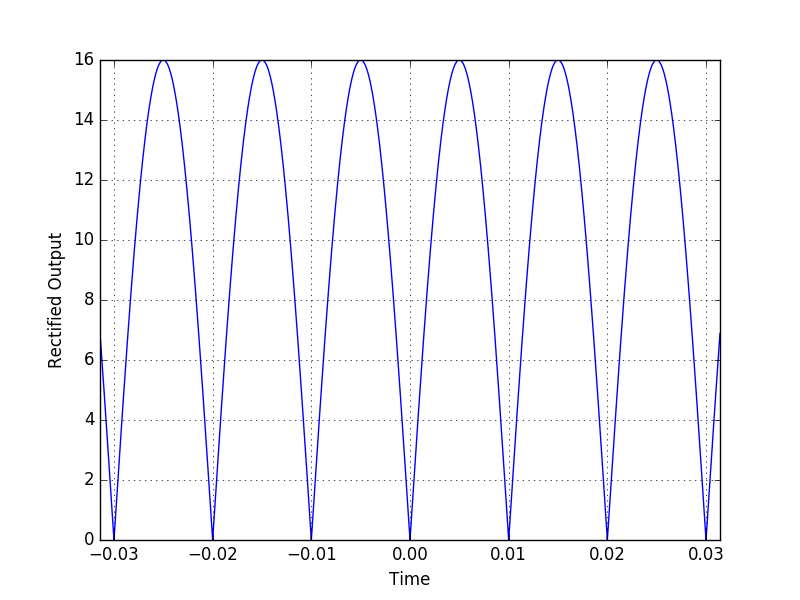
\includegraphics[scale=0.4]{./figs/expectedrectified.png}
	\caption{Expected Rectified Wave}  \label{recex}
    \end{figure}





\section{Fourier Analysis}
\begin{problem}
Find the frequency and amplitude of the not rectified wave.
\end{problem}
\solution
The frequency is 50 Hz and amplitude is approximately 16 V.
\begin{problem}
The following expression
%
\begin{equation}
g(t) = \sum_{n=0}^{\infty}a_n\cos 2\pi n f t + b_n \sin 2 \pi n f t
\end{equation}
is known as the Fourier series expansion of $g(t)$, where $f = \frac{1}{T}$.  Find 
\begin{align}
a_n &= \frac{2}{T} \int_{0}^{T}g(t) \cos 2\pi nf t \, dt \\
b_n &= \frac{2}{T} \int_{0}^{T}g(t) \sin 2\pi nf t \, dt
\end{align}
Using this find the fourier series coefficients of the rectified outputs.
\end{problem}
%
\solution 
\begin{align}
a_0 &= \frac{2A}{\pi}\\
&=\frac{32}{\pi}
\end{align}
and
\begin{align}
a_n &= \frac{-2A}{\pi(4n^2-1)}
\end{align}
Similarly, 
\begin{align}
b_n & = 0
\end{align}

\begin{problem}
Write a code for the plotting the same graph as that in problem 1.1
\end{problem}
\solution
\lstinputlisting[language=Python]{./codes/fourierrectified.py}

\begin{figure}[h]
\centering
	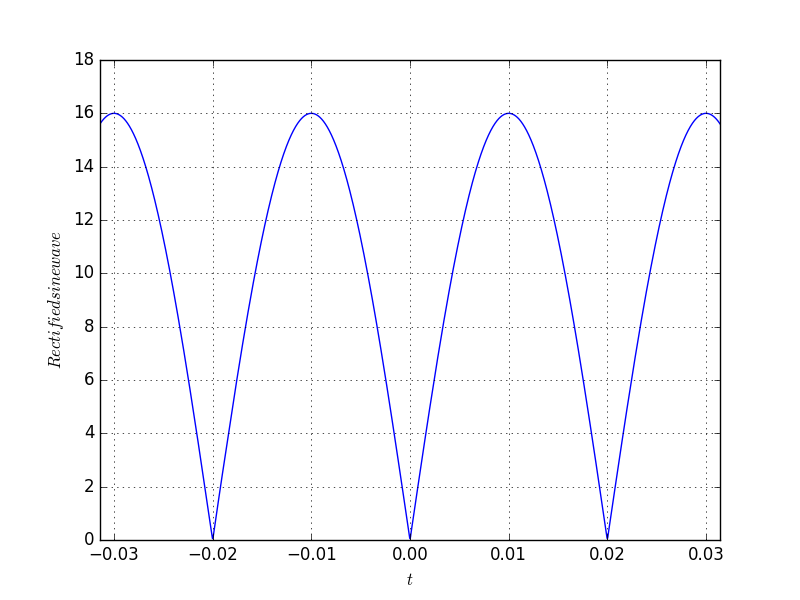
\includegraphics[scale=0.4]{./figs/fourierrectified.png}
	\caption{Rectified Wave from fourier series}  \label{recf}
    \end{figure}


\section{Rectified Ac to Dc}
%\begin{problem}
%What is the role of the capacitor in the circuit?
%\end{problem}
%\solution
%The output of the diode bridge is a DC consisting of ripples also called as pulsating DC. This pulsating DC can be filtered using an inductor filter or a capacitor filter or a resistor-capacitor-coupled filter for removing the ripples. Consider a capacitor filter which is frequently used in most cases for smoothing.
\begin{problem}
Type the following code in python to plot the amplitude of the frequencies present in the rectified wave.
\end{problem}
\lstinputlisting[language=Python]{./codes/frequency.py}
\solution
The output is as shown in the Fig. \ref{frequencies.png}
\begin{figure}[h]
\centering
	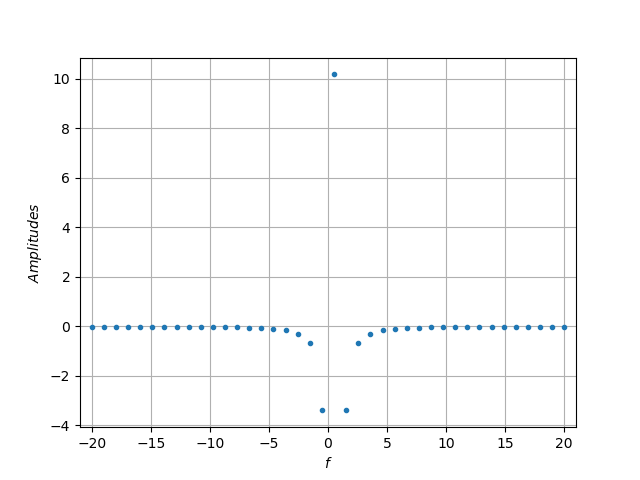
\includegraphics[scale=0.4]{./figs/frequencies.png}
	\caption{Frequencies}  \label{frequencies}
    \end{figure}

\begin{problem}
Find the response of the RC filter used.
\end{problem}
\solution
The RC response can be shown to be as folows.
\begin{align}
H(s) &= \frac{1}{\brak{sCR + 1 }}
\label{lpf_laplace}
\end{align}
\begin{align}
\abs{H(s)} &= \frac{1}{\sqrt{\brak{(sCR)^2 + 1 }}} \\
\label{lpf1laplace}
\end{align}
\begin{problem}
Substitute $s = \jmath 2\pi f, \jmath =  \sqrt{-1}$ in Equation 3.2.1 to obtain $H(f)$.  
$H(f)$ is 
known as the frequency response.  Given that $R = 1 \Omega$ and $C = 1000 \,\mu F$.
\end{problem}
%

\begin{problem}
The given figure \ref{fig3} contains 2 plots. Blue graph is  a plot of fourier series coeffiecients of rectified AC wrt frequency. The orange plot is the frequency response of an RC circuit. We have used a capacitor of 1000uf and Resistance is very low(it is mainly due to wires only).The peak of the graph is at 0 and at other points, it decays exponentially. So it works as a low pass filter and only thfrequencies near 0 frequencies are passed. Thus we get DC output. 


\begin{figure}[h]
\centering
	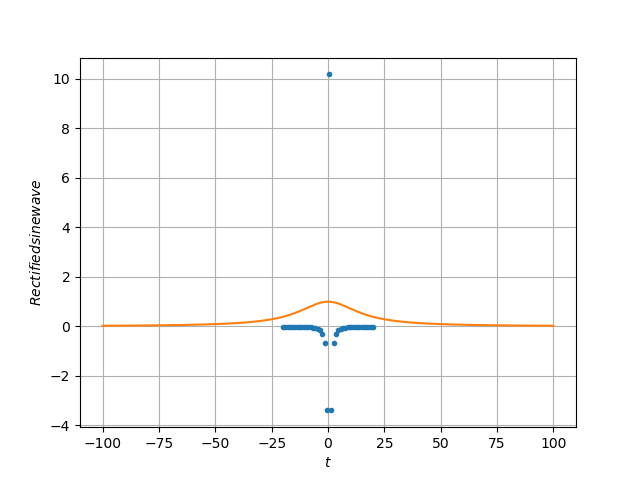
\includegraphics[scale=0.4]{./figs/dc.png}
	\caption{Rectified Wave with Capacitive filter}  \label{fig3}
    \end{figure}
\end{problem}
\section{Final Output}
Final Output will look like the red part Fig. 4.0
\begin{figure}[h]
\centering
	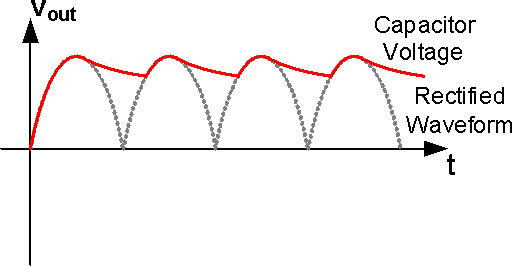
\includegraphics[scale=0.4]{./figs/cap.png}
	\caption{DC }  \label{fig5}
    \end{figure}




\end{document}
